\documentclass[12pt,xcolor=table,aspectratio=169]{beamer}
\usetheme{Frankfurt}
\usecolortheme{rose}
\usepackage{amsthm}
\usepackage{amsmath}
\usepackage{bbm}
\usepackage{amsfonts}
\usepackage{amssymb}
\usepackage{graphicx}
\usepackage{hyperref}
\usepackage[flushleft]{threeparttable}
\usepackage{tabularx}
\usepackage{booktabs}
\usepackage{siunitx}
\usepackage{tikz}
\usetikzlibrary{decorations.pathreplacing,angles,quotes}
%\usepackage{enumitem}% http://ctan.org/pkg/enumitem

%set up course and number

\newcommand{\ClassName}{TBD}
\newcommand{\ClassNumber}{TBD}
\newcommand{\Topic}{TBD}

% Some optional colors. Change or add as you see fit.
%---------------------------------------------------
 \definecolor{ualbertagreen}{HTML}{007C41}
\definecolor{ualbertagold}{HTML}{FFDB05}

\definecolor{calloutgrey}{HTML}{D9D9D9}


%set fonts
\setbeamerfont{subtitle}{size=\large,shape=\scshape,series=\bfseries}
\setbeamerfont{title}{size=\Large,shape=\scshape,series=\bfseries}
\setbeamerfont{author}{size=\large}
\setbeamerfont{date}{size=\large}
\setbeamerfont{caption}{size=\scriptsize}


% Some optional color adjustments to Beamer. Change as you see fit.
%------------------------------------------------------------------
\setbeamercolor{frametitle}{fg=ualbertagreen,bg=white}
\setbeamercolor{title}{fg=ualbertagreen,bg=white}
\setbeamercolor{author}{fg=ualbertagreen,bg=white}
\setbeamercolor{date}{fg=ualbertagreen,bg=white}
\setbeamercolor{local structure}{fg=ualbertagreen}
\setbeamercolor{section in toc}{fg=ualbertagreen,bg=white}
% \setbeamercolor{subsection in toc}{fg=ualbertagreen,bg=white}
\setbeamercolor{footline}{fg=ualbertagreen!50, bg=white}

% definition boxes
\setbeamercolor{block title}{bg=ualbertagreen,fg=white}
\setbeamercolor{block body}{parent=normal text,use=block title,bg=calloutgrey}
%\setbeamercolor{block body}{parent=normal text,use=block title,bg=block title.bg!30!bg}


\setbeamercolor{upper separation line head}{bg=ualbertagreen}
\setbeamercolor{lower separation line head}{bg=ualbertagold}
\setbeamercolor{middle separation line head}{bg=ualbertagold}
\setbeamercolor{frametitle}{fg=ualbertagreen,bg=white}



\setbeamercolor{section in head/foot}{bg=white,fg=ualbertagreen}
\setbeamercolor{author in head/foot}{bg=white,fg=ualbertagreen}
\setbeamercolor{date in head/foot}{bg=white,,fg=ualbertagreen}
\setbeamercolor{title in head/foot}{bg=white,fg=ualbertagreen}

\setbeamercolor{headline}{bg=white,fg=ualbertagreen}




\setbeamercolor*{middle separation line head}{bg=ualbertagreen}
\setbeamercolor*{alerted text}{fg=ualbertagreen}
\setbeamercolor*{example text}{fg=black}
\setbeamercolor*{structure}{fg=black}


\let\Tiny=\tiny



\logo{
   %\ifnum\insertpagenumber>1
   \tikz [remember picture,overlay]
    \node[yshift=.3cm,xshift=1.5cm] at (current page.south west)
        %or: (current page.center)
        {
\includegraphics[width=1in]{../images/UA-ASB-COLOUR.png}};
    %\fi
%
\includegraphics[height=0.8cm]{../images/UA-ASB-COLOUR.png}\vspace{220pt}
}


\setbeamertemplate{title page}{%
  \vbox{}
    \vspace{.5cm}% NEW
  \begingroup
    \centering
    \begin{beamercolorbox}[sep=8pt,center]{title}
      \usebeamerfont{title}\ClassNumber: \ClassName\par%
      \usebeamerfont{title}\inserttitle\par%
     \ifx\insertsubtitle\@empty%
      \else%
        \vskip0.05em%
        {\usebeamerfont{subtitle}\usebeamercolor[fg]{subtitle}\insertsubtitle\par}%
      \fi%
    \end{beamercolorbox}%
    \begin{beamercolorbox}[sep=8pt,center]{author}
      \usebeamerfont{author}\insertauthor
    \end{beamercolorbox}
    \begin{beamercolorbox}[sep=8pt,center]{institute}
      \usebeamerfont{institute}\insertinstitute
    \end{beamercolorbox}

    \vspace{0.5cm}% NEW
    \begin{beamercolorbox}[sep=8pt,center]{date}
      \usebeamerfont{date}\insertdate
    \end{beamercolorbox}\vskip0.05em

      \endgroup
  %\vfill
}


\setbeamertemplate{frametitle}{%
    \insertframetitle\par\vskip-10pt
}



\renewcommand{\ClassName}{Business Economics, Organization and Management}
\renewcommand{\ClassNumber}{BUEC 311}

\setbeamertemplate{headline}{%
\leavevmode%
 \hbox{%
    \begin{beamercolorbox}[wd=\paperwidth,ht=5ex,dp=0ex]{white}%
    \usebeamerfont{headline}\hskip6pt\ClassNumber: \inserttitle\par%
    \insertsectionnavigationhorizontal{\paperwidth}{}{\hskip0pt plus1filll}
    \end{beamercolorbox}%
  }
}

\defbeamertemplate*{footline}{my footline}{%
    \ifnum\insertpagenumber=1
        \Tiny{%
            \hfill%
		\vspace*{1pt}%
            %\insertframenumber/\inserttotalframenumber \hspace*{0.1cm}%
            \newline%
            \color{ualbertagold}{\rule{\paperwidth}{0.4mm}}\newline%
            \color{ualbertagold}{\rule{\paperwidth}{.4mm}}%
        }
  \else%
        \Tiny{%
            \hspace{.66\paperwidth}
            %\vspace{25pt}
            \insertframenumber/\inserttotalframenumber
            \newline%
            \color{ualbertagold}{\rule{\paperwidth}{0.4mm}}\newline%
            \color{ualbertagold}{\rule{\paperwidth}{.4mm}}%
        }%
    \fi%
}


\newenvironment{itemize*}%
  {\begin{itemize}%
    \setlength{\itemsep}{0pt}%
    \setlength{\parskip}{0pt}}%
  {\end{itemize}}


\title{Strategic Behaviour Part 2\\
	Strategies Over Time and Dynamic Games
}

\date{Fall 2021}

\begin{document}

\section{Overview}

\frame{
	\titlepage
}


\frame{
	\frametitle{Strategic Interaction Over Time}
	\begin{itemize}
	\item Last topic: Strategic interaction in static setting.
		\begin{itemize}
		\item But in practice, many interactions occur \underline{dynamically} over time.
		\end{itemize}
	\item[]
	\item \underline{Dynamic games}: Games where players play the game over and over, and move either \underline{repeatedly} or \underline{sequentially}.
	\end{itemize}
}


\frame{
	\frametitle{Outline}
	\begin{enumerate}
	\item Repeated Games
	\item[]
	\item Sequential Games
	\item[]
	\item Deterring Entry
	\item[]
	\item Cost and Innovation Strategies
	\item[]
	\item Disadvantages of Moving First
	\item[]
	\item Behavioural Game Theory
	\end{enumerate}
}

\section{Repeated Games}

\frame{
	\frametitle{Outline}
	\begin{enumerate}
	\item \alert{Repeated Games}
	\item[]
	\item Sequential Games
	\item[]
	\item Deterring Entry
	\item[]
	\item Cost and Innovation Strategies
	\item[]
	\item Disadvantages of Moving First
	\item[]
	\item Behavioural Game Theory
	\end{enumerate}
}

\frame{
	\frametitle{Repeated Games}
	\begin{itemize}
	\item A repeated game is a game in which a static \textit{constituent} game is repeated a finite and pre-specified number of times, or is repeated indefinitely.
	\item[]
	\item We still need to know:
		\begin{itemize}
		\item Players
		\item Rules
		\item Information
		\item Payoffs
		\end{itemize}
	\item[]
	\item Key difference from a static game: How we think about actions and strategies.
	\end{itemize}
}

\frame{
	\frametitle{Repeated Games}
	\begin{itemize}
	\item In a repeated game:
		\begin{itemize}
		\item An \underline{action} is a single move that a player makes at a specified time, such as choosing an output level or a price.
		\item[]
		\item A \underline{strategy} is a battle plan that specifies the \textit{full set} of actions that a player will make throughout the game.
			\begin{itemize}
			\item It may involve actions that are conditional on prior actions of other players, or on new information available at a given time.
			\end{itemize}
		\end{itemize}
	\end{itemize}
}

\frame{
	\frametitle{Repeated Games}
	\begin{itemize}
	\item As an example, we will revisit game between American and United.
	\item[]
	\item Recall: The Nash equilibrium in the static game is both firms producing high (64k passengers) and making \$4.1 million.
	\end{itemize}
}

\frame{
	\frametitle{Repeated Games}
	\begin{figure}
	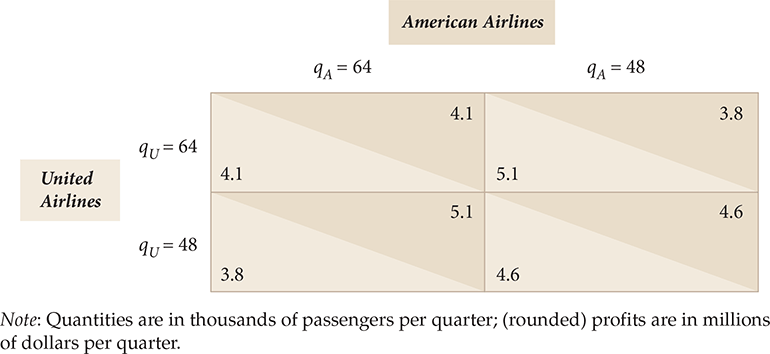
\includegraphics[scale=0.4]{../images/game_theory/oligopoly.png}
	\end{figure}
}

\frame{
	\frametitle{Repeated Games}
	\begin{itemize}
	\item Now assume that the same game gets \underline{repeated indefinitely}.
		\begin{itemize}
		\item Now firms must consider both current and future profits.
		\end{itemize}
	\item[]
	\item With repetition, the outcome may be different than in the static game.
		\begin{itemize}
		\item Depends on the strategies used by the firms.
		\end{itemize}
	\end{itemize}
}

\frame{
	\frametitle{Repeated Games}
	\begin{itemize}
	\item Suppose, for example, that American adopts the following strategy:
		\begin{itemize}
		\item It cheap-talks United that it will produce the collusive or cooperative quantity of 48k in the first period.
		\item But its subsequent decisions depend on United:
			\begin{itemize}
			\item If United produces 48k in period $t$, American will produce 48k in period $t+1$.
			\item If United produces 64k in period $t$, American will produce 64k in period $t+1$.
			\end{itemize}
		\end{itemize}
	\item[]
	\item What is United's best response to this strategy?
	\end{itemize}
}

\frame{
	\frametitle{Repeated Games}
	\begin{figure}
	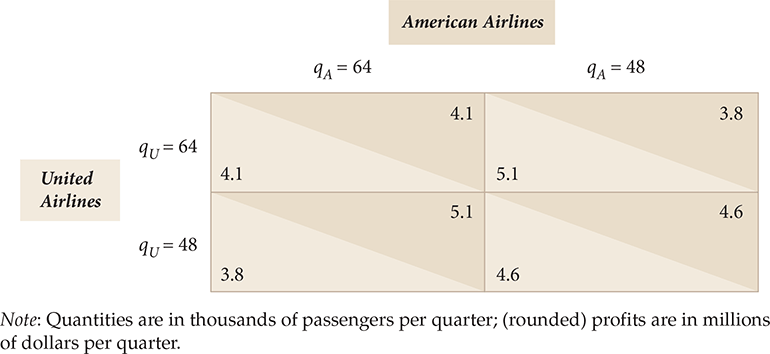
\includegraphics[scale=0.4]{../images/game_theory/oligopoly.png}
	\end{figure}
}

\frame{
	\frametitle{Repeated Games}
	\begin{itemize}
	\item American's strategy is an example of a \underline{trigger strategy}.
		\begin{itemize}
		\item Trigger strategy: Rival's defection from a collusive outcome \textit{triggers} punishment.
		\end{itemize}
	\item[]
	\item If United adopts the same trigger strategy, the Nash-equilibrium is the collusive outcome.
		\begin{itemize}
		\item Neither firm has an incentive to deviate.
		\item One period gains from doing so are not sufficient to offset all future losses.
		\end{itemize}
	\item[]
	\item In reality, cooperation may not be sustainable because of regulation, bounded rationality, or if the firm cares little about future profits.
	\end{itemize}
}

\frame{
	\frametitle{Repeated Games}
	\begin{itemize}
	\item Trigger strategy is just one possible option for American.
	\item[]
	\item They could instead adopt a \underline{tit-for-tat} strategy.
		\begin{itemize}
		\item Tit-for-tat: Cooperate in first round, then copy rival's action in each subsequent round.
		\end{itemize}
	\item[]
	\item Tit-for-tat may induce cooperation if the payoff from deviating in any period is less than the loss from punishment in the subsequent period.
		\begin{itemize}
		\item It depends on how firms discount the future.
		\end{itemize}
	\item[]
	\item Cooperation is also more likely if the tit-for-tat strategy is modified to extend punishment for more than one period.
		\begin{itemize}
		\item Extension of punishment needs to offset the one-time gains from not cooperating.
		\end{itemize}
	\end{itemize}
}

\frame{
	\frametitle{Repeated Games}
	\begin{itemize}
	\item The equilibrium of the repeated game between American and United is an example of a collusive outcome.
	\item[]
	\item In most modern economies, explicit collusion is illegal.
		\begin{itemize}
		\item However, antitrust and competition laws typically do not strictly prohibit choosing the cooperative (or cartel) quantity or price as long as no \underline{explicit} agreement is reached.
		\item Firms may be able to engage in \underline{implicit collusion} or \underline{tacit collusion} using trigger, tit-for-tat, or other similar strategies, as long as firms do not explicitly communicate with each other.
			\begin{itemize}
			\item Tacit collusion lowers society's total surplus just as explicit collusion does.
			\end{itemize}	
		\end{itemize}
	\end{itemize}
}

\frame{
	\frametitle{Repeated Games}
	\begin{itemize}
	\item Sustaining the cooperative outcome requires that players believe the game will repeat for ever.
	\item[]
	\item if there is a known end to the game, and players have complete foresight, the cooperation can be impossible to maintain.
	\end{itemize}
}

\frame{
	\frametitle{Repeated Games}
	\begin{itemize}
	\item  To see this, suppose that American and United know that they will play the game a finite number of times ($T$).
	\item[]
	\item Suppose both firms use the trigger strategy that sustained collusion when the game was infinitely repeated.
	\item[]
	\item Now, the trigger strategy does not lead to a Nash Equilibrium.
	\item[]
	\item Why not?
	\end{itemize}
}

\frame{
	\frametitle{Repeated Games}
	\begin{figure}
	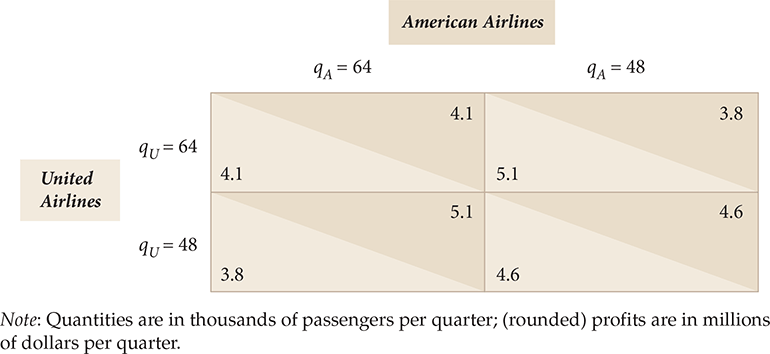
\includegraphics[scale=0.4]{../images/game_theory/oligopoly.png}
	\end{figure}
}

\frame{
	\frametitle{Repeated Games}
	\begin{itemize}
	\item When the game is repeated a finite number of times, the only Nash Equilibrium is for both firms to produce a high level of output in all periods.
		\begin{itemize}
		\item There is no cooperation again.
		\end{itemize}
	\end{itemize}
}

\section{Sequential Games}

\frame{
	\frametitle{Outline}
	\begin{enumerate}
	\item Repeated Games
	\item[]
	\item \alert{Sequential Games}
	\item[]
	\item Deterring Entry
	\item[]
	\item Cost and Innovation Strategies
	\item[]
	\item Disadvantages of Moving First
	\item[]
	\item Behavioural Game Theory
	\end{enumerate}
}

\frame{
	\frametitle{Sequential Games}
	\begin{itemize}
	\item So far, we've maximized strategic interactions where players make simultaneous decisions.
	\item[]
	\item But in many interactions, players alternate moves.
	\item[]
	\item We can model this type of strategic interaction as a \underline{sequential game}.
	\end{itemize}
}

\frame{
	\frametitle{Stackelberg Oligopoly}
	\begin{itemize}
	\item As an example, we will again revisit the interaction between American and United, but we will now assume that the firms move sequentially in two stages:
		\begin{itemize}
		\item First, American (the \underline{leader}) chooses its output level.
		\item Second, United (the \underline{follower}) chooses its output level.
		\end{itemize}
	\item[]
	\item This is an example of a \underline{Stackelberg} oligopoly.
		\begin{itemize}
		\item Stackelberg oligopoly involves one leader and one or more followers.
		\end{itemize}
	\end{itemize}
}

\frame{
	\frametitle{Stackelberg Oligopoly}
	\begin{figure}
	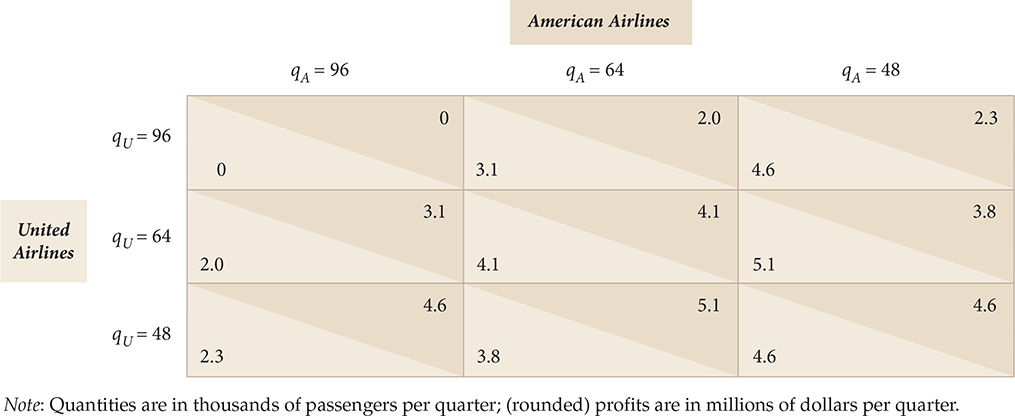
\includegraphics[scale=0.35]{../images/game_theory/stackelberg.png}
	\caption{Payoffs in the Stackelberg game}
	\end{figure}
}

\frame{
	\frametitle{Decision trees}
	\begin{itemize}
	\item Key issue with the payoff matrix:
		\begin{itemize}
		\item It does not show the sequential nature of the game.
		\end{itemize}
	\item[]
	\item We can better illustrate the game using an extensive form diagram.
		\begin{itemize}
		\item Also known as a game tree, or a decision tree.
		\item The extensive form is a branched diagram that shows the players, the sequence of moves, the actions players can take at each move, the information that each player has about previous moves, and the payoff function over all possible strategy combinations.
		\end{itemize}
	\end{itemize}
}

\frame{
	\frametitle{Stackelberg Game Tree}
	\begin{figure}
	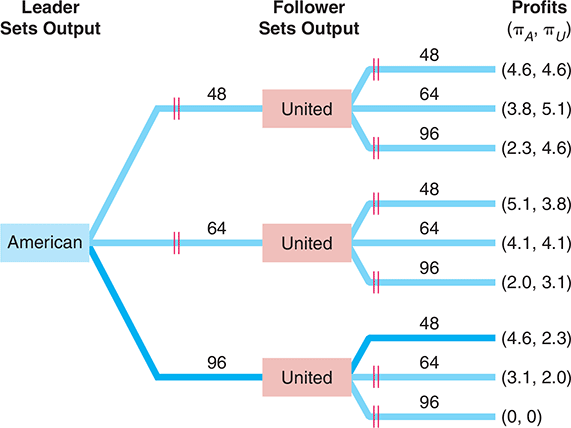
\includegraphics[scale=0.4]{../images/game_theory/stackelberg_tree.png}
	\end{figure}
}

\frame{
	\frametitle{Subgames}
	\begin{itemize}
	\item The sequential game depicted in the extensive form has four \underline{subgames}.
	\item[]
	\end{itemize}
	\begin{definition}[Subgame]
	A subgame consists of all of the actions (and the corresponding payoffs) that a player can take at a given stage in the game, \textit{given the actions that have already been taken}.
	\end{definition}
}

\frame{
	\frametitle{Subgame Perfection}
	\begin{itemize}
	\item To predict the outcome of the sequential game, we need to know the set of strategies that form a Nash equilibrium in each subgame.
		\begin{itemize}
		\item These strategies yield the \underline{subgame-perfect Nash Equilibrium}.
		\end{itemize}
	\item[]
	\item We can solve for the subgame-perfect Nash Equilibrium through backward induction.
		\begin{itemize}
		\item First, we determine the best response by the last player to move, then we determine the best response for the player who makes the next-to-last move, and so on, until we reach the first move of the game.
		\end{itemize}
	\end{itemize}
}

\frame{
	\frametitle{Subgame Perfection}
	\begin{figure}
	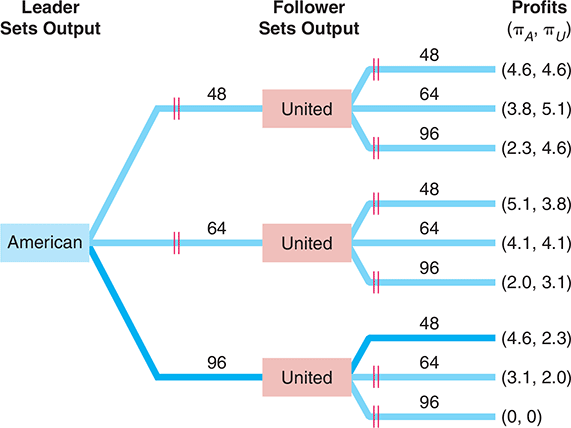
\includegraphics[scale=0.4]{../images/game_theory/stackelberg_tree.png}
	\end{figure}
}

\frame{
	\frametitle{Subgame Perfection}
	\begin{itemize}
	\item In the game between American and United, American first determines what United (the follower), will do in the second stage of the game in each of the three subgames.
		\begin{itemize}
		\item This is the $q_U$ with the highest profit at each node.
		\end{itemize}
	\item[]
	\item American then determines the best action in the first stage given the choices that United will make \textit{conditional on its actions} in the second stage.
		\begin{itemize}
		\item This amounts to choosing the $q_A$ with the highest profit.
		\end{itemize}
	\item[]
	\item Thus, American chooses $q_A = 96$ in the first stage, and United chooses $q_U =48$ in the second stage.
		\begin{itemize}
		\item This is a subgame perfect Nash equilibrium; neither firm wants to change its strategy given what the other player is doing.
		\end{itemize}
	\end{itemize}
}

\frame{
	\frametitle{Simultaneous vs. Sequential Games}
	\begin{itemize}
	\item It is worth noting that if this game was played simultaneously, the Nash equilibrium would be $q_{A}=q_{U}=64$.
	\item[]
	\item Simultaneous and sequential games have different solutions because of credible threats and first mover advantage.
		\begin{itemize}
		\item For a firm's strategy to be a \underline{credible threat}, rivals must believe that the firm's strategy is rational (that is, it works in the firm's best interest).
		\item In the simultaneous move game between United and American, United will not believe a threat by American to produce 96. However, in the sequential game, commitment to produce 96 is credible because American makes the first move.
		\end{itemize}
	\end{itemize}
}



\frame{
	\frametitle{Other Examples}
	\begin{itemize}
	\item Entry Deterrence
    \item Sports - a golf or tennis match
    \item Limit pricing
    \item Innovation and R\&D
    \item Bargaining
    \end{itemize}
}


\end{document}

